\section{Gjennomføring med måleresultater}

\subsection{Krets 1 -- enveis klippekrets}
\begin{figure}[H]
\centering
\begin{tikzpicture}
\begin{axis}[
    width=11cm,
    axis lines=middle,
    xlabel={$t\:[ms]$},
    ylabel={$V\:[V]$},
    xmin=0, xmax=6.5,
    ymin=-12, ymax=12,
    samples=400,
    domain=0:6.28,
    ytick={-10,-5,0.8,5,10},
    yticklabels={$-10$, $-5$, $0.800$, $5$, $10$},
    xtick={3.14,6.28},
    xticklabels={$10$, $20$},
    legend style={
        at={(0.98,0.98)},
        anchor=north east,
        draw=none,
        fill=none
    }
]

% Inngangsspenning
\addplot[
    blue,
    thick
] {10*sin(deg(x))};
\addlegendentry{$V_{in}$}

\addplot[
    red,
    thick,
    domain=3.14:6.28
] {10*sin(deg(x))};

% Utgangsspenning med styrt, glatt klipping
\addplot[
    red,
    thick,
    smooth,
] coordinates {
    (0.00, 0.00)
    (0.01, 0.10)
    (0.02, 0.20)
    (0.03, 0.30)
    (0.04, 0.40)
    (0.06, 0.45)
    (0.09, 0.50)
    (0.13, 0.56)
    (0.18, 0.62)
    (0.24, 0.67)
    (0.31, 0.71)
    (0.39, 0.74)
    (0.47, 0.77)
    (0.55, 0.79)
    (0.63, 0.80)
};
\addlegendentry{$V_{out}$}

\addplot[
    red,
    thick
] coordinates {(0.63, 0.80) (2.51, 0.80)};

\addplot[
    red,
    thick,
    smooth,
] coordinates {
    (2.51, 0.80)
    (2.55, 0.795)
    (2.59, 0.79)
    (2.67, 0.77)
    (2.75, 0.74)
    (2.83, 0.71)
    (2.90, 0.67)
    (2.96, 0.62)
    (3.01, 0.56)
    (3.05, 0.50)
    (3.08, 0.45)
    (3.10, 0.40)
    (3.11, 0.30)
    (3.12, 0.20)
    (3.13, 0.10)
    (3.14, 0.00)
};

% Horisontal hjelpelinje ved klippenivå
\addplot[
    dashed,
    gray
] coordinates {(0,0.8) (6.28,0.8)};

\end{axis}
\end{tikzpicture}
\caption{Måleresultat for krets 1.}\label{fig:resultat_krets1}
\end{figure}

\subsection{Krets 2 -- toveis klippekrets}
\begin{figure}[H]
\centering
\begin{tikzpicture}
\begin{axis}[
    width=11cm,
    axis lines=middle,
    xlabel={$t\:[ms]$},
    ylabel={$V\:[V]$},
    xmin=0, xmax=6.5,
    ymin=-12, ymax=12,
    samples=400,
    domain=0:6.28,
    ytick={-10,-5,-0.8,0.8,5,10},
    yticklabels={$-10$, $-5$, $-0.800$, $0.800$, $5$, $10$},
    xtick={3.14,6.28},
    xticklabels={$10$, $20$},
    legend style={
        at={(0.98,0.98)},
        anchor=north east,
        draw=none,
        fill=none
    }
]

% Inngangsspenning
\addplot[
    blue,
    thick
] {10*sin(deg(x))};
\addlegendentry{$V_{in}$}

% -------- POSITIV HALVPERIODE --------

\addplot[
    red,
    thick,
    smooth
] coordinates {
    (0.00, 0.00)
    (0.01, 0.10)
    (0.02, 0.20)
    (0.03, 0.30)
    (0.04, 0.40)
    (0.06, 0.45)
    (0.09, 0.50)
    (0.13, 0.56)
    (0.18, 0.62)
    (0.24, 0.67)
    (0.31, 0.71)
    (0.39, 0.74)
    (0.47, 0.77)
    (0.55, 0.79)
    (0.63, 0.80)
};

\addplot[
    red,
    thick
] coordinates {(0.63, 0.80) (2.51, 0.80)};

\addplot[
    red,
    thick,
    smooth
] coordinates {
    (2.51, 0.80)
    (2.55, 0.795)
    (2.59, 0.79)
    (2.67, 0.77)
    (2.75, 0.74)
    (2.83, 0.71)
    (2.90, 0.67)
    (2.96, 0.62)
    (3.01, 0.56)
    (3.05, 0.50)
    (3.08, 0.45)
    (3.10, 0.40)
    (3.11, 0.30)
    (3.12, 0.20)
    (3.13, 0.10)
    (3.14, 0.00)
};

% -------- NEGATIV HALVPERIODE (speilet) --------

\addplot[
    red,
    thick,
    smooth
] coordinates {
    (3.14, 0.00)
    (3.15, -0.10)
    (3.16, -0.20)
    (3.17, -0.30)
    (3.18, -0.40)
    (3.20, -0.45)
    (3.23, -0.50)
    (3.27, -0.56)
    (3.32, -0.62)
    (3.38, -0.67)
    (3.45, -0.71)
    (3.53, -0.74)
    (3.61, -0.77)
    (3.69, -0.79)
    (3.77, -0.80)
};

\addplot[
    red,
    thick
] coordinates {(3.77, -0.80) (5.65, -0.80)};

\addplot[
    red,
    thick,
    smooth
] coordinates {
    (5.65, -0.80)
    (5.69, -0.795)
    (5.73, -0.79)
    (5.81, -0.77)
    (5.89, -0.74)
    (5.97, -0.71)
    (6.04, -0.67)
    (6.10, -0.62)
    (6.15, -0.56)
    (6.19, -0.50)
    (6.22, -0.45)
    (6.24, -0.40)
    (6.25, -0.30)
    (6.26, -0.20)
    (6.27, -0.10)
    (6.28, 0.00)
};

% Klippelinjer
\addplot[dashed, gray] coordinates {(0,0.8) (6.28,0.8)};
\addplot[dashed, gray] coordinates {(0,-0.8) (6.28,-0.8)};

\addlegendentry{$V_{out}$}

\end{axis}
\end{tikzpicture}
\caption{Måleresultat for krets 2.}\label{fig:resultat_krets2}
\end{figure}

\subsection{Krets 3 -- zenordioder i klippekrets}

\subsection{Krets 3}
\begin{figure}[H]
\centering
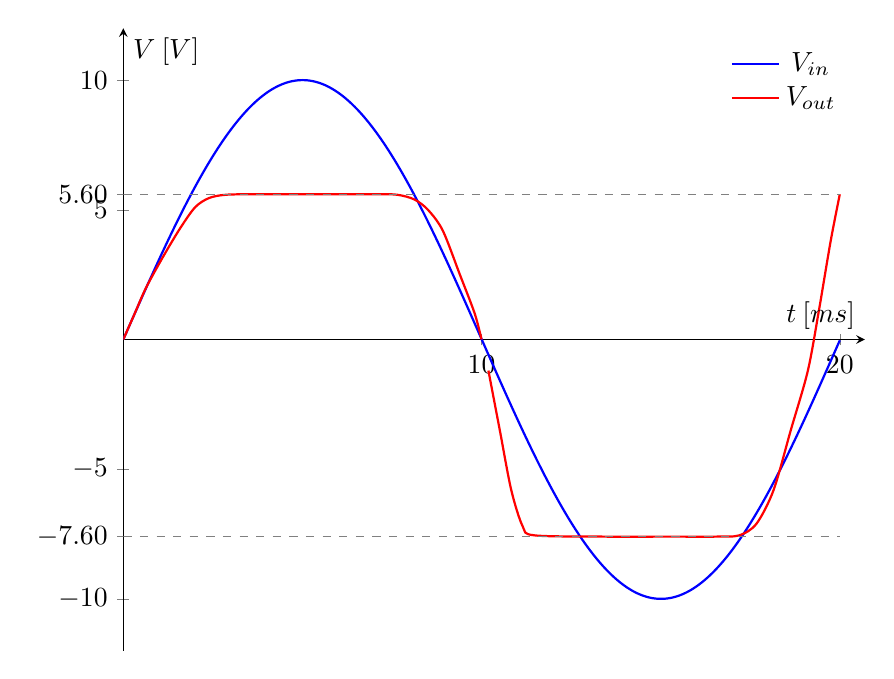
\begin{tikzpicture}
\begin{axis}[
    width=11cm,
    axis lines=middle,
    xlabel={$t\:[ms]$},
    ylabel={$V\:[V]$},
    xmin=0, xmax=6.5,
    ymin=-12, ymax=12,
    samples=400,
    domain=0:6.28,
    ytick={-10,-7.60,-5,0,5,5.60,10},
    yticklabels={$-10$, $-7.60$, $-5$, $0$, $5$, $5.60$, $10$},
    xtick={3.14,6.28},
    xticklabels={$10$, $20$},
    legend style={
        at={(0.98,0.98)},
        anchor=north east,
        draw=none,
        fill=none
    }
]

% Inngangsspenning
\addplot[
    blue,
    thick
] {10*sin(deg(x))};
\addlegendentry{$V_{in}$}

% Utgangsspenning
\addplot[
    red,
    thick,
    smooth
] coordinates {
    % Positiv halvperiode
    (0.00, 0.00)
    (0.10, 1.00)
    (0.20, 2.00)
    (0.35, 3.20)
    (0.50, 4.30)
    (0.63, 5.10)
    (0.75, 5.45)
    (0.90, 5.58)
    (1.20, 5.60)
    (1.80, 5.60)
    (2.20, 5.60)
    (2.40, 5.58)
    (2.55, 5.40)
    (2.67, 5.00)
    (2.80, 4.20)
    (2.95, 2.50)
    (3.08, 1.00)
    (3.14, 0.00)

    % Negativ halvperiode
    (3.20, -1.20)
    (3.30, -3.50)
    (3.40, -5.80)
    (3.50, -7.20)
    (3.60, -7.55)
    (4.20, -7.60)
    (4.80, -7.60)
    (5.20, -7.60)
    (5.40, -7.55)
    (5.55, -7.10)
    (5.70, -5.80)
    (5.85, -3.50)
    (6.00, -1.20)
    (6.10, 1.20)
    (6.20, 3.80)
    (6.28, 5.60)
};
\addlegendentry{$V_{out}$}

% Hjelpelinjer
\addplot[
    dashed,
    gray
] coordinates {(0,5.60) (6.28,5.60)};

\addplot[
    dashed,
    gray
] coordinates {(0,-7.60) (6.28,-7.60)};

\end{axis}
\end{tikzpicture}
\caption{Måleresultat for krets 3. Utgangsspenningen får en asymmetrisk klipping, med toppverdi omtrent $5.60\,\mathrm{V}$ og bunnverdi omtrent $-7.60\,\mathrm{V}$.}
\label{fig:resultat_krets3}
\end{figure}

\subsection{Krets 4 -- enveis likeretter}

\subsection{Krets 5 -- toveis likeretter}

\subsection{Krets 6 -- toveis likeretter med kondensator}